%%TODO: IF THIS GETS IN, CITE MY THESIS (since I present an early version
%of this idea in my background and copied some text from there)

% Template for ICIP-2018 paper; to be used with:
%          spconf.sty  - ICASSP/ICIP LaTeX style file, and
%          IEEEbib.bst - IEEE bibliography style file.
% --------------------------------------------------------------------------
\documentclass{article}
\usepackage{spconf,amsmath,amssymb,amsfonts,amsthm,graphicx}

\usepackage{tikz}

\graphicspath{{Figures/}}
\newcommand{\argmin}{\operatornamewithlimits{argmin}}
\newcommand{\argmax}{\operatornamewithlimits{argmax}}
\newcommand{\matt}[1]{{\color{purple}[MSB: #1]}}
\newcommand{\mb}{\mathbf}


\title{Topological Eulerian Synthesis of Slow Motion Periodic Videos}

%
% Single address.
% ---------------
\name{Author(s) Name(s)\thanks{Thanks to XYZ agency for funding.}}
\address{Author Affiliation(s)}
%
% For example:
% ------------
%\address{School\\
%	Department\\
%	Address}
%
% Two addresses (uncomment and modify for two-address case).
% ----------------------------------------------------------
%\twoauthors
%  {A. Author-one, B. Author-two\sthanks{Thanks to XYZ agency for funding.}}
%	{School A-B\\
%	Department A-B\\
%	Address A-B}
%  {C. Author-three, D. Author-four\sthanks{The fourth author performed the work
%	while at ...}}
%	{School C-D\\
%	Department C-D\\
%	Address C-D}
%
\begin{document}
%\ninept
%
\maketitle
%


\begin{abstract}

The majority of our pipeline is fully automated, using tools from topological data analysis in concert with nonlinear dimenison reduction to autotune the spatial and temporal scales of the period.

\end{abstract}
%
\begin{keywords}
One, two, three, four, five
\end{keywords}
%


\section{Introduction}
%Background, drift, noise, large motion, static pixels, scale finding, overall automation [fundamental frequency, etc].  Sliding window "time regularization"

Repetitive, periodic behavior is ubiquitous in our world. Animal locomotion, mechanical motion, biological rhythms, and musical rhythms can all be characterized as periodic phenomena.  In this work, we consider the problem of taking a video that contains such repetitive motion of many periods, and synthesizing a single fine detail, slow motion template cycle.  This fine detailed analysis can be applied, for example, to characterize subtle progressions of blood flow in the face during a heartbeat \cite{kumar2015distanceppg}.  Having access to a consensus template can also be used to visualize variations from cycle to cycle. This could be used to indicate the onset of failure in a repetitive automated action on an assembly line, to assess the stress of motions in repetitive human actions~\cite{greene2017visualizing}, and to optimize performance in athletic activities.

Our approach to slow motion templates is {\em Eulerian}; that is, we process the video pixel by pixel with no tracking.  Eulerian approaches for video synthesis are attractive due to their simplicity and ease of implementation.  For instance, a simple Fourier bandpass filtering and amplifying pixels can successfully elucidate subtle periodic motions in videos \cite{wu2012eulerian, wadhwa2013phase}.  Additionally, time domain Eulerian approaches have been used to synthesize infinitely playing ``video textures'' using random walks \cite{schodl2000video}, or to synthesize perfectly looping video templates after grouping pixels with similar periods together and devising a common period for all groups \cite{Liao2013VideoLoops,Liao2015VideoLoops}.  There are some pitfalls with Eulerian techniques, however.  They are known to fail for large motions, and also require the user to manually specify frequencies of interest \cite{wu2012eulerian, wadhwa2013phase}.  Furthermore, period-to-period drift that is due to a moving camera or small variation in motion can be problematic, as well as unrelated motion in the background \cite{stauffer1999adaptive}.

% MSB: opportunity to slim paper by cutting examples 
To address the problems with an Eulerian representation, we devise a geometric/topological Eulerian framework by constructing {\em sliding window embeddings} of videos (Section~\ref{sec:slidingwindow}).  Sliding window embeddings, or delay reconstructions, have found a diverse array of applications in activity recognition \cite{frank2010activity,venkataraman2016shape}, gene expression data \cite{perea2015sw1pers}, EEG analysis \cite{stam2005nonlinear, plesnik2014detection}, audio and music analysis \cite{herzel1994analysis,serra2009cross,bello2011measuring,traliemoebius}, video analysis \cite{tralie2017quasi}, and motion capture analysis \cite{venkataraman2016shape}.  Sliding window embeddings of periodic time series, in particular, form samples of a topological loop \cite{perea2015sliding}, as do generalized multivariate sliding windows on periodic video data, regardless of the type of motion present \cite{traliehigh, tralie2017quasi}.  Furthermore, the sliding window embedding of an Eulerian video provides a form of regularization that mitigates the effects of drift and leads to a cleaner loop~\cite{tralie2017quasi}.  Our geometric framework also allows us to use topological data analysis \cite{edelsbrunner2000topological,edelsbrunner2008persistent,edelsbrunner2010computational,carlsson2009topology,ghrist2014elementary} and fundamental frequency estimation \cite{Mcleod05asmarter} to autotune the spatial and temporal scales of the periodic motion, respectively, so that no user intervention is required.  We use Laplacian Eigenmaps~\cite{belkin2003laplacian} computed on the sliding window embedding to obtain a circular phase $\phi \in [0, 2\pi]$ for each window.  The video is re-ordered by using $\phi$ and exploiting the sliding window structure, where different windows vote on the final pixels in each frame of the template, helping to further mitigate drift (Section~\ref{sec:cyclereordering}).  As an illustration, Figure~\ref{fig:ConceptFigure} shows an example of our technique on a sampled periodic time series (i.e. single pixel grayscale video).  There are only 12 samples per period in the original signal, so the details of each period are coarse and noisy.  However, once they are re-sorted, we get a fine-detailed representation of one period.  The extension of this technique to videos will be described in detail in Section~\ref{sec:methods}.


% MSB: opportunity to slim paper by cutting examples 
Many prior works use a combination of sliding window embeddings and topological data analysis, such as detecting the Lorenz attractor \cite{de2012topological}, quantifying circadian rhythms in gene expression data \cite{perea2015sliding}, detecting chatter in mechanical systems \cite{khasawneh2016chatter}, detecting wheezing in audio \cite{emrani2014real}, quantifying periodic activites in motion capture data \cite{vejdemo2015cohomological, venkataraman2016persistent}, and quantifying vocal fold anomalies in video \cite{tralie2017quasi}, though we believe we are the first to use a sliding window + TDA framework to {\em synthesize} a new result. Related works have used the graph Laplacian to rearrange images around a loop as a pre-processing step for structure from motion \cite{averbuch2015ringit}, and to reorder the frames of microscope images from a developing embryo around a loop using vector diffusion maps~\cite{dsilva2015diffusionvecordering}.  However, our use of the graph Laplacian to instead {\em parameterize} time series is unique. One can also view the combination of TDA + Laplacian eigenmaps as a simpler alternative to cohomology circular coordinates \cite{de2011persistent,vejdemo2015cohomological} for the special case of periodic data.  It is also the opposite of the approach in \cite{bendich2011improving}, which performs diffusion maps before TDA. \matt{unclear what ''It'' refers to in this last sentence}


\section{Slow Motion Templates}
\label{sec:methods}

\begin{figure*}[h!]
\centering
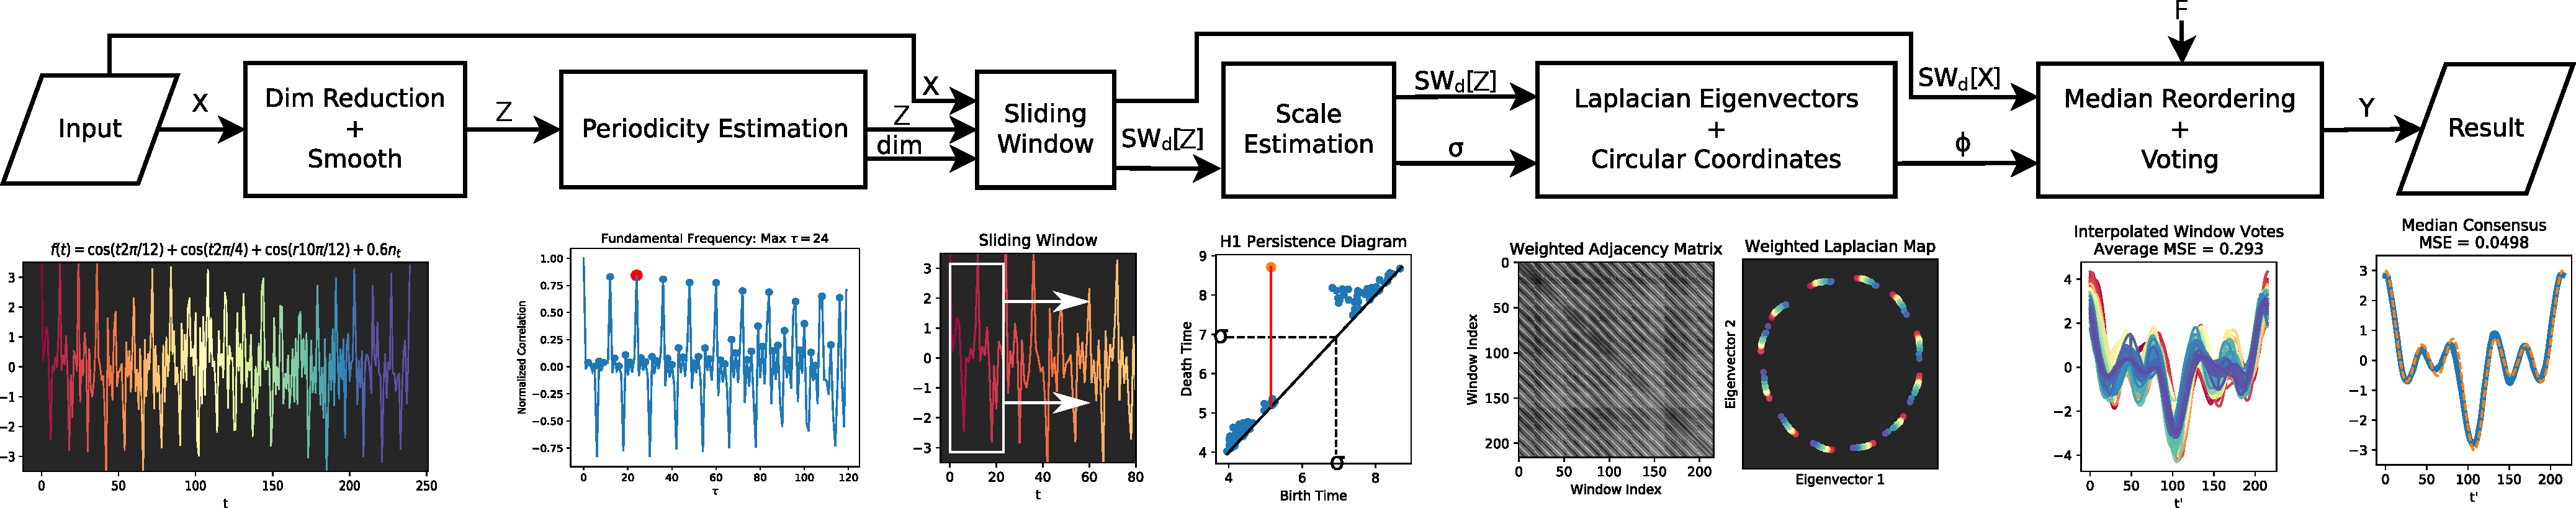
\includegraphics[width=\textwidth]{BlockDiagram.pdf}
\caption{An block diagram of our technique, illustrated by a 1D periodic time series with additive Gaussian noise ($n_t \in \mathcal{N}(0, 1)$).  We estimate the period to be 24 (a multiple of the fundamental frequency), and perform a 24-length sliding window embedding.  From this, we use the mean of the birth and death time of the largest persistence dot to autotune the scale $\sigma$ for the graph Laplacian, from which we derive circular coordinates $\phi$, which can be used to reorder the sliding windows and use them to vote on a final slow motion template.  The result is shown in the bottom rightmost plot, superimposed with a ground truth period shown as an orange dotted line.}
\label{fig:ConceptFigure}
\end{figure*}

Figure~\ref{fig:ConceptFigure} depicts an overview of our method. First we estimate the period of the cycle, and use this to compute the sliding window embedding (a). Next we estimate the spatial scale of the embedding using persistent homology (b). Given the scale, we then compute a single-cycle reordering of the embedding using Laplacian Eigenmaps (c). Last, we use the reordered embedding to reorder the original video through median voting of windows (d).

\textbf{Preprocessing.} The input to our method is a 3-channel video of $N$ frames, each frame of resolution $W \times H$. We treat each frame as a point in Euclidean space of dimension $\mathbb{R}^{3 \cdot W \cdot H}$, and denote the set of all videos by the sequence $\mb{X}(t) \in \mathbb{R}^{(3 \cdot W \cdot H)}$ for integer-valued $t \in [1,N]$. The steps of our approach outlined in Figure~\ref{fig:ConceptFigure}(a-c), however, do not rely on the {\em extrinsic} geometry of the set of points $\mb{X}(t)$, only its set of {\em pairwise distances}. Thus, we can project all of the points into a lower-dimensional space and apply the set of techniques to the projection, assuming that pairwise distances are preserved. Since $N \ll (3 \cdot W \cdot H)$, the frames can be projected into a $N-1$-dimensional space such that all distances are preserved. Denoting this projection by $\mb{P} \in \mathbb{R}^{(N-1) \times (3 \cdot W \cdot H)}$, our method for steps (a)-(c) operates on $\mb{Z}(t) = \mb{P} \mb{X}(t)$.

%We now describe our algorithm in several stages.  Throughout our discussion, we assume we are given 3 channel color videos with $W \times H$ resolution frames, so that each frame is a Euclidean vector in $\mathbb{R}^{W \times H \times 3}$.  For a video with $N$ frames, we flatten each frame to a 1D vector and stack them row wise along an $N \times 3WH$ matrix $X$.  Whenever we perform a linear operation on all of the pixels at once, we can use the SVD $X = USV^T$ to reduce memory and computational costs by working with $US$ in place of $X$, which is in $N$ dimensions instead of $3WH \gg N$ (similar processing was done in \cite{turk1991eigenfaces} and \cite{tralie2017quasi}).  The only nonlinear operation is the median operation (Section~\ref{sec:cyclereordering}), and we project back into pixel space using $V^T$ before taking the median.

\subsection{Sliding Window Embeddings}
\label{sec:slidingwindow}

The sliding window video embedding \cite{cao1998dynamics,traliehigh,tralie2017quasi} for $\mb{Z}$ can defined as
\begin{equation}
	SW_{D}[\mb{Z}(t)] = \left[ \begin{array}{c} \mb{Z}(t) \\ \mb{Z}(t + 1) \\ \vdots \\ \mb{Z}(t + (D-1))  \end{array} \right] \in \mathbb{R}^{(N-1)\cdot(D)},
\end{equation}
where D is the dimension of the embedding. As shown by Takens~\cite{takens1981detecting}, a sliding window of dimension $2m+1$ of even a single generic observation function of a dynamical system of intrinsic dimension $m$ is sufficient to reconstruct a topological embedding of the underlying trajectory in the original state space.  For periodic signals, this state space is a torus, and $d$ should be twice the number of harmonics present to injectively reconstruct loops on that torus \cite{perea2015sliding}.  The same is true of videos in general \cite{tralie2017quasi}.  Furthermore, the sliding window length $(D-1)$ maximizes the roundness of the embeddings when $(D-1) = k T$ for some integer $k$, where $T$ is the fundamental period.  Since we will use topological data analysis (TDA) to find the scale of the loop, and since TDA measures roundness, it is important that we tune our window size to be an integer multiple of the period.  To do this, we perform 1D ISOMAP \cite{tenenbaum2000global} on the original frames of the video to generate a 1D surrogate signal, and we perform an autocorrelation-based fundamental frequency estimation \cite{Mcleod05asmarter} on this signal to estimate the period and, hence, the appropriate $D$.  This is similar to the diffusion maps + autocorrelation approach in \cite{tralie2017quasi} for analyzing periodic videos.  This estimation often returns integer multiples of the fundamental period, which is fine for our purposes.
% MSB: could probably remove the diffusion maps + autocorrelation approach sentence if we need space

\subsection{Laplacian Eigenmaps}
\label{sec:laplacian}

\begin{figure}[h!]
\centering
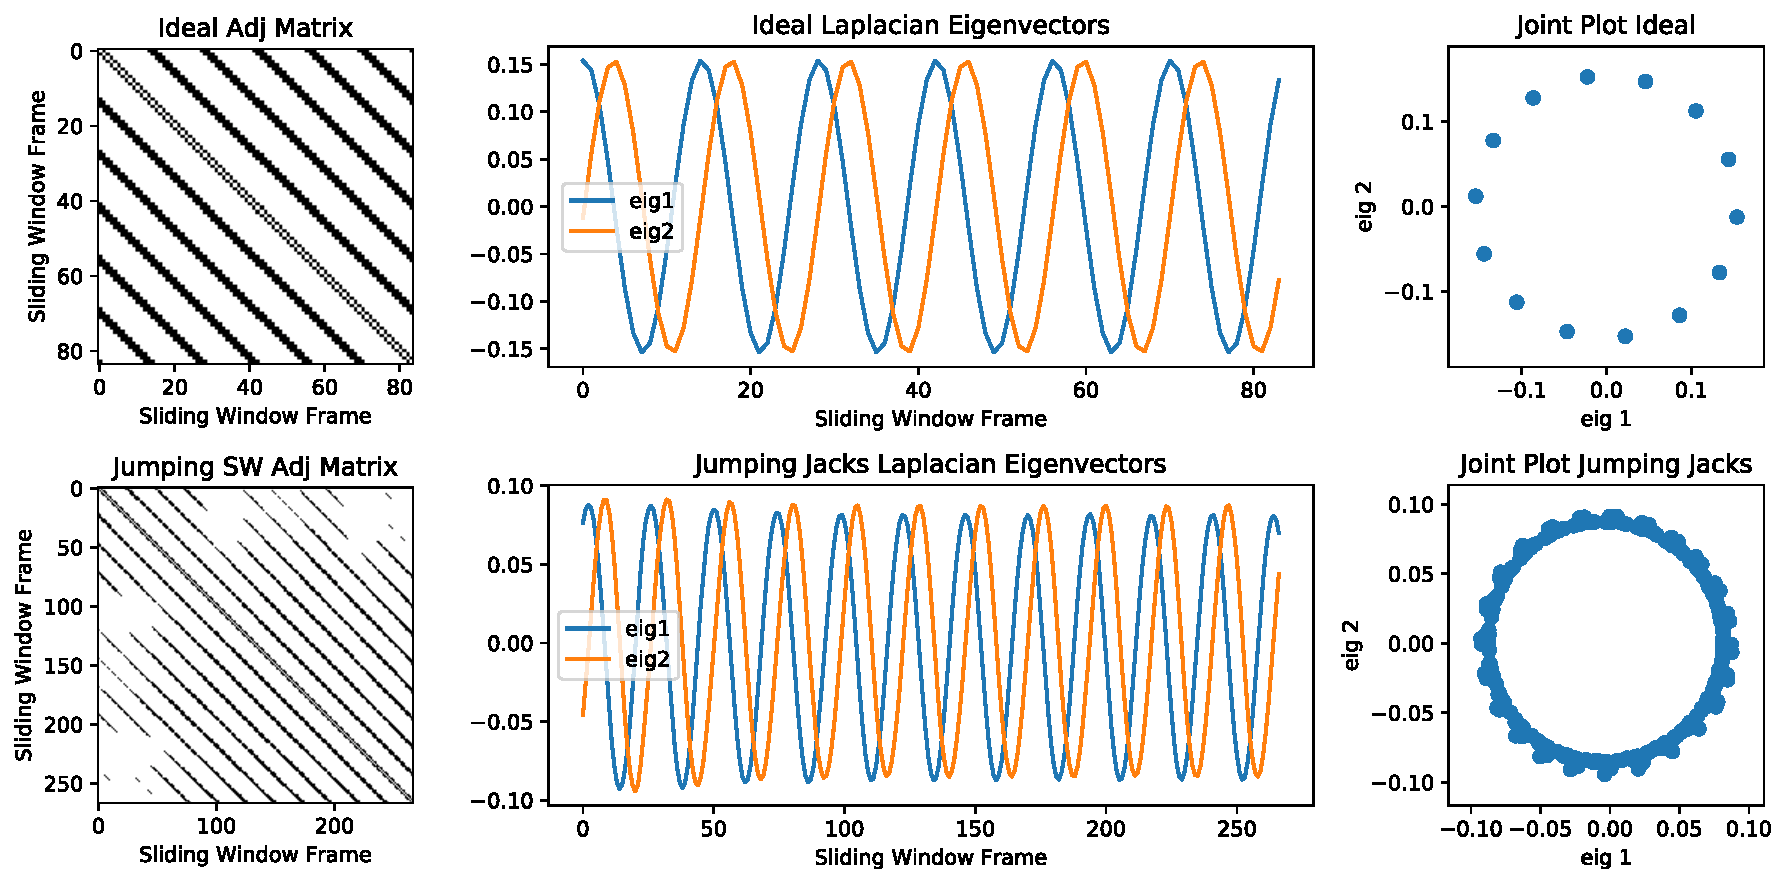
\includegraphics[width=\columnwidth]{CirculantExample.pdf}
\caption{An example of the unweighted graph Laplacian on an ideal adjacency matrix corresponding to 6 periods of length 14 (top row), and the adjacency matrix from a sliding window embedding of two men doing jumping jacks (bottom row).  }
\label{fig:CirculantExample}
\end{figure}
%The two eigenvectors corresponding the smallest nonzero eigenvalues of the graph Laplacian span sinusoids that are 90 degrees out of phase, and which reconstruct a circle when plotted against each other.

Since sliding window embeddings of periodic videos lie on a topological loop, this means that, at an appropriate scale, a nearest neighbors graph built on the sliding window point cloud will approximately be a graph representing a circle.  To parameterize this graph, we turn to the graph Laplacian \cite{chung1997spectral}. To define the graph Laplacian, we first construct an adjacency matrix $\mb{A}$ in which the entry at $\mb{A}_{ij}$ represents the similarity between windows at times $i$ and $j$: $\mb{A}_{ij} = exp(-||SW_{D}[\mb{Z}(i)] - SW_{D}[\mb{Z}(j)]||_2/\epsilon)$. The graph Laplacian then follows as:
\begin{equation}
	\mb{L} = \mb{D}-\mb{A}
\end{equation}
where $\mb{D}_{ii} = \sum_{j = 1}^N \mb{A}_{ij}, \mb{D}_{i \neq j} = 0$ is the diagonal matrix.  Now let $d_{ij}: V \rightarrow \mathbb{R}^+$ be a nonnegative scalar function on the vertices of $G$.  Then the adjacency matrix correponding to the unweighted graph Laplacain, $A_{\epsilon}^u(d)$, is

\begin{equation}
A_{\epsilon}^u(d)_{ij} = \left\{ \begin{array}{cc} 1 & i \neq j, d_{ij} \leq \epsilon \\ 0 & \text{otherwise} \end{array} \right\}
\end{equation}

Alternatively, the weighted adjacency matrix is defined as $A_{\epsilon}^w(d)_{ij} = \exp(-d_{ij}^2/\epsilon)$ \cite{belkin2003laplacian}, but everything else is the same.  Now suppose we have performed a sliding window $SW_{D}[X[n]]$ for a video $X$, where $X[n] = X[n+kT]$ for some integers $l, k$ so that there are $kT$ points in the sliding window (that is, $SW_{D}[X[i]]$ repeats itself exactly every $T$ frames $k$ times total, for a total of $N = kT$ windows), and that $d_{ij} = ||SW_{D}[X[i]] - SW_{D}[X[j]]||_2$.  In this case, for any $\epsilon > 0$ and $|i - j| = kT$ for some integer $k$, $A^u_{\epsilon}(d)_{ij} = 1$.  Let us further suppose it is possible to choose an $\epsilon$ so that each window is also connected to the window directly before and after it in time, as well as the windows directly before and after its repetitions, but none others; that is, the unweighted adjacency matrix is a symmetric, {\em circulant matrix}, with the first row $A_{\epsilon}^u(d)_{1j} = 1$ if $j = 1, N-1,$ or $lT, 1 \leq l \leq (k-1)$.  Thus, the Laplacian is also circulant with first row

\begin{equation}
\label{eq:modellaplacian}
L_{1j} = \left\{ \begin{array}{cc} 3k-1 & j = 1 \\ -1 & j = lT, 1 \leq l \leq (k-1) \\ -1 & j = 1, N-1 \\ 0 & \text{otherwise} \end{array} \right\}
\end{equation}

Circulant matrices are diagonalized by the Discrete Fourier Transform \cite{godsil2013algebraic}, and their nonzero eigenvalues come in pairs with multiplicity two, with corresopnding eigenvectors $v_1[n] = 1$, $v_{2m}[n] = \cos(2 \pi mn / N)$, $v_{2m+1}[n] = \sin(2 \pi m n / N)$, $m \geq 1$.  In the case of Equation~\ref{eq:modellaplacian}, it can be shown using the DFT that the eigenvalues are $\lambda_1 = 0$ and 

\begin{equation}
\begin{array}{cc}\lambda_{2m},\\\lambda_{2m+1}\end{array} = \left\{ \begin{array}{cc} 3k - k\left( 1 + 2 \cos \left( \frac{2 \pi}{kT} m \right) \right) & m = lk, l \in \mathbb{Z}^+ \\ 3k & \text{otherwise}  \end{array} \right\} 
\end{equation}

The smallest two nonzero eigenvalues occur when $m = k$, corresponding to the eigenvectors \footnote{This generalizes the circle graph used in \cite{averbuch2015ringit}, in which $T = N, k = 1$} 
\begin{equation}
v_{2k}[n] = \cos(2 \pi n / T), v_{2k+1}[n] = \sin(2 \pi n / T)
\end{equation}
When computing the smallest two nonzero eigenvalues numerically, therefore, one coresponds to a sinusoid with period $T$, and the other to an orthogonal sinusoid with period $T$.  When plotted against each other, they form a circle, with an arbitrary phase offset.  Therefore, we compute the circular phase numerically $\phi = \tan^{-1}(\hat{v_1}[n] / \hat{v_2}[n])$, where $\hat{v_i}$ is the eigenvector corresponding to the $i^\text{th}$ smallest nonzero numerical eigenvalue.  In practice, the graphs we get from sliding window may deviate from the ideal Laplacian model in Equation~\ref{eq:modellaplacian}, though they do so gracefully.  Figure~\ref{fig:CirculantExample} shows an example of $\hat{v_1}[n]$ and $\hat{v_2}[n]$ for an ideal graph and for an imperfect graph corresponding to the sliding window embedding of a real video.  

Note that for both the unweighted and weighted cases in practice, we have observed that harmonics of the actual frequency of interest occasionally have smaller eigenvalues.  To mitigate this, we use the pair of eigenvectors with the smallest number of zero crossings within the eigenvectors corresponding to the 10 smallest nonzero eigenvalues.

\subsection{Persistent Homology}
Our discussion so far has assumed we can find the appropriate $\epsilon$ for the (un)weighted graph Laplacian, but this is data dependent.
%The authors of \cite{averbuch2015ringit} use $k$-nearest neighbors, which helps with scale, but which still requires an arbitrary parameter $k$.
To adapt to the data, we leverage 1D persistent homology from topological data analysis \cite{edelsbrunner2010computational}.  This framework allows one to find the scale at which topological features exist in point cloud data.  Specifically, we compute the 1D Vietoris Rips Filtration on our sliding window data $X$, which tracks equivalence classes of loops, known as {\em homology classes} \cite{Hatcher}, as edges and triangles are gradually added between sliding window points.  The algorithm returns a so-called persistence diagram, which is a multiset of points on a 2D birth/death grid, with each point corresponding to a loop class.  The birth value $b_i$ indicates the scale at which the $i^{\text{th}}$ loop class forms, and the death value $d_i$ indicates the scale at which that class no longer exists (expressible as a formal sum of triangle boundaries with coefficients in some field).  The difference $d_i - b_i$ is known as the {\em persistence} of the $i^{\text{th}}$ class.  For sliding window periodic time series, one point in the diagram should have a much larger persistence than the others (e.g. Figure~\ref{fig:ConceptFigure})~\cite{perea2015sliding,tralie2017quasi}, and this ideally reflects the single cycle of motion that we seek.  We take our scale to be $\frac{1}{2}(b_i + d_i)$ for the largest $d_i - b_i$. % MSB: last sentence might change based on experiments

Finally, homology computation requires the specification of coefficients that belong to a user-given field. Coefficients in $\mathbb{Z}_2$ are commonly chosen, however in our scenario this is problematic. For instance, the motion of someone performing a jumping jack contains a second harmonic, since an individual jumps twice per cycle, and using coefficients in $\mathbb{Z}_2$ would lead to so-called M{\"o}bius splitting~\cite{traliemoebius}. Thus, we use coefficients in the field $\mathbb{Z}_{49}$ in order to capture these types of complex motions.
% MSB: mention use of software in experiments, not in techniques

%Finally, note that we compute homology using $\mathbb{Z}_{49}$ coefficients to handle cases where a period has strong harmonics, since, choosing a field which is not relatively prime to a harmonic leads to lowered persistence \cite{perea2015sliding, traliemoebius}.  For instance, a jumping jacks motion has a second harmonic, since an individual jumps twice per cycle, so the common persistence algorithm with $\mathbb{Z}_2$ coefficients would lead to ``M{\"o}bius splitting'' \cite{traliemoebius}.  We use the GUDHI library\cite{maria2014gudhi} to compute persistent homology quickly with fields other than $\mathbb{Z}_2$.

\subsection{Cycle Reordering And Median Voting}
\label{sec:cyclereordering}



Advantage of Eulerian is that everything is linear (can use SVD to compress)

Interpolated windows can be projected back to pixel space one by one to save memory

Mention the ``F'' parameter in the pipeline

\section{Experiments}

\subsection{Robustness Tests}


\begin{figure}
\centering
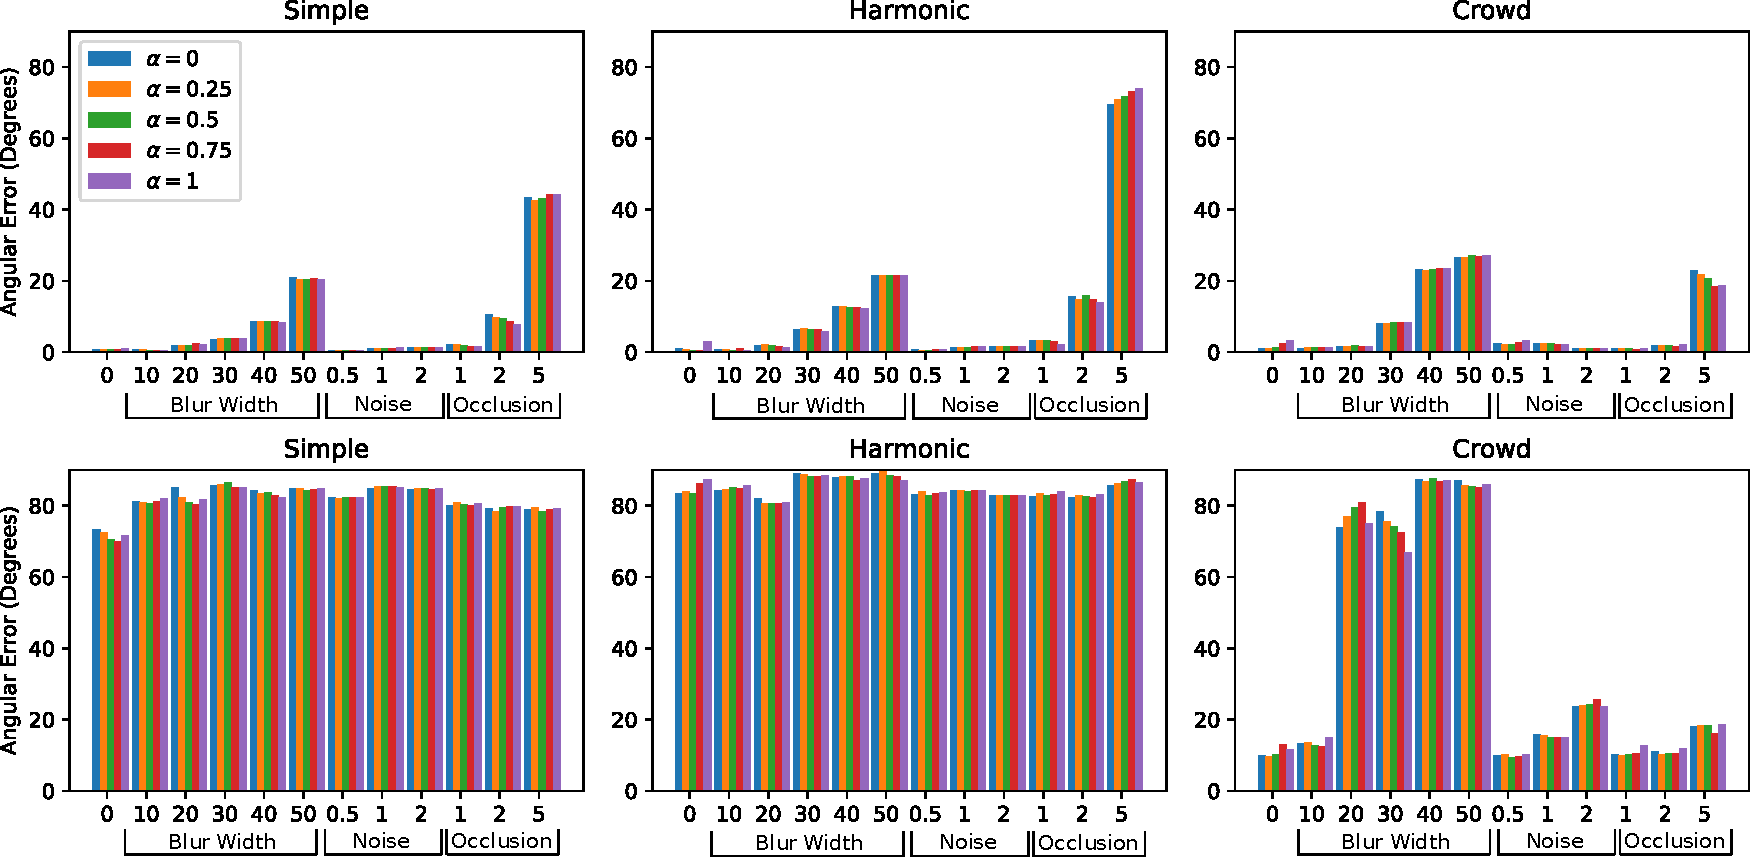
\includegraphics[width=\columnwidth]{RobustnessTests.pdf}
\caption{Robustness tests.}
\label{fig:RobustnessTests}
\end{figure}

\begin{figure}
\centering
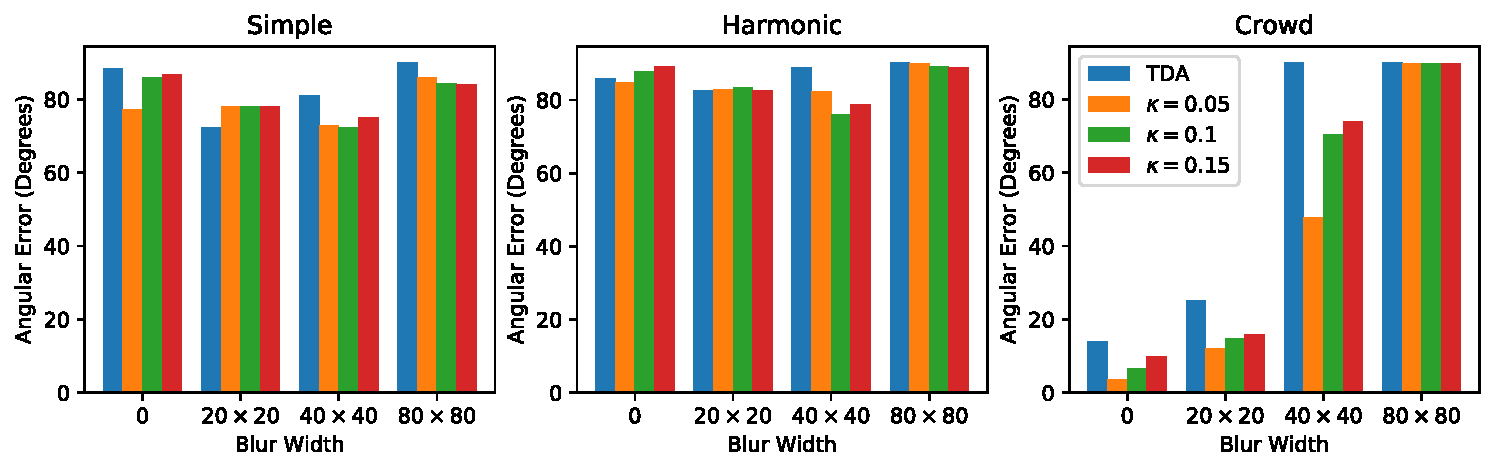
\includegraphics[width=\columnwidth]{RobustnessTestsNoSW.pdf}
\caption{Robustness tests without sliding window.}
\label{fig:RobustnessTestsNoSW}
\end{figure}


We now experimentally quantify the accuracy of our circular coordinate inference, since we cannot hope to get a good slow motion template unless our circular coordinates are accurate.  We generate 3 different 600 frame synthetic periodic videos for which we know the ground truth circular coordinates, using software from \cite{jacobson2012fast}.  We vary the number of cycles that the videos undergo between 3, 5, 10, 15, 20, 25, 30, 40, and 50, and we also vary the ``shake'' of the video (width of a motion blur kernel) from 0, $20 \times 20$, $40 \times 40$, and $80 \times 80$, to assess the effect of drift.  We also compare different fractions $\kappa$ of mutual nearest neighbors to tune the threshold at which the unweighted Laplacian is built to TDA for aututuning the scale.  Figure~\ref{fig:RobustnessTests} shows the average angular error in degrees for our entire pipeline, and Figure~\ref{fig:RobustnessTests}.  The errors are overall quite low for moderate shake with a sliding window, though they increase as more shake is introduced.  Without a sliding window, the only video that performs reasonably well is the ``crowd'' videom, though the errors increase with shake much more rapidly than with the sliding window, supporting the ``time regularization'' properties of the sliding window.


\subsection{Qualitative Results}
\begin{figure}
\centering
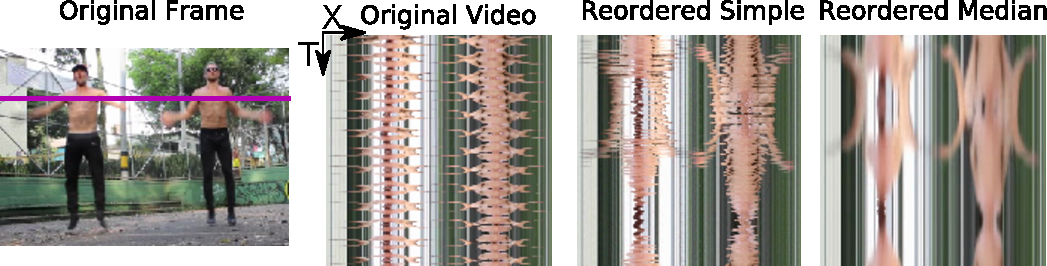
\includegraphics[width=\columnwidth]{XTSliceJumpingJacks.pdf}
\caption{An XT slice of a line of pixels (magenta line, upper left) over time for an input video of two men doing jumping jacks and for reordered videos with and without median consensus.}
\label{fig:XTSliceJumpingJacks}
\end{figure}

\begin{figure}
\centering
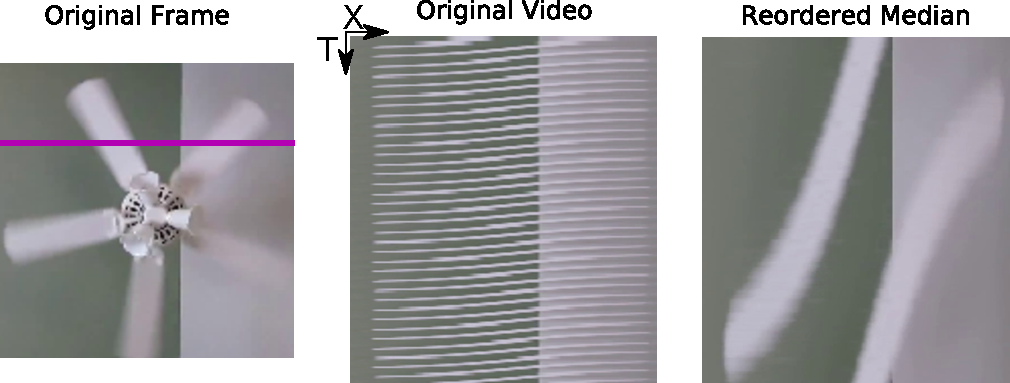
\includegraphics[width=\columnwidth]{XTSliceFan.pdf}
\caption{An XT slice of a line of pixels (magenta line, upper left) over time for an input video of a fan with only 6 frames per period and the corresponding median consensus reordered video.}
\label{fig:XTSliceFan}
\end{figure}

We now qualitatively examine the results of our slow motion templates on some examples.  Figure~\ref{fig:XTSliceJumpingJacks} shows the difference between a simple reordering and a median consensus reordering.  Due to natural variation from cycle to cycle, the simple reordering has many temporal discontinuities when interleaving these cycles.  By contrast, the median voting is clean, and it has the added benefit of removing nonperiodic background components.  Figure~\ref{fig:XTSliceFan} shows an extreme example in which an original spinning fan video has only 6 frames per period at framerate.  In addition to these examples, in our supplementary material, we show results from jumping jacks 2 men, two exercise videos from \cite{levy2015live}, and beating heart videos from \cite{traliehigh}, \cite{wu2012eulerian}, and \cite{wadhwa2013phase}.

\section{Discussion}

Since we rely on the theory and constructions in \cite{tralie2017quasi}, we are subject to similar constraints in the allowable motion and drift for our method to work well.  We note that Eulerian video magnification also degrades in the presence of too much drift \cite{wu2012eulerian, wadhwa2013phase}.


% References should be produced using the bibtex program from suitable
% BiBTeX files (here: strings, refs, manuals). The IEEEbib.bst bibliography
% style file from IEEE produces unsorted bibliography list.
% -------------------------------------------------------------------------
\bibliographystyle{IEEEbib}
\bibliography{refs}

\end{document}
